\documentclass[11pt]{my_memo}
\usepackage{longtable,booktabs,array}
\usepackage{graphicx}
\usepackage[hyphens]{url}
% a case name may break after an underscore or a slash
\newcommand{\case}[1]{\seqsplit{#1}}
\usepackage{seqsplit}
% The text block is the class default; the wide tables are set one font size
% down so that a case name still stands on one line.
\setlength{\tabcolsep}{3pt}
\renewcommand{\arraystretch}{1.0}
\title{The LHS 1140 b catalog: what is certified and what is not}
\author{EXHALE}
\date{2026-09-22}
\begin{document}
\maketitle

\noindent
Every model of the catalog is LHS 1140 b on 500 cells, solved by the
partitioned stationary route with \texttt{Well balanced: True}, from the
GJ~1132 spectrum placed at this planet's orbit. The binary of record is
\texttt{EXHALE\_75d55d9d.x}, md5 \texttt{75d55d9d4fd0e748cd01d6e35713e34c},
and the counts below are MEASURED by \texttt{models/status.py inventory},
re-run read-only at 2026-09-22 11:55:41 KST: \textbf{143 state indexes, 92
certified}, the same totals the stored \texttt{CASE\_INVENTORY.json} carries
from its 2026-09-21 21:10 reading. A case counts as certified when its index
names a \texttt{latest\_certified} generation that no refused re-evaluation
has marked stale. Section 3 and section 4 list the 94 models of the ladders
and of \texttt{diffusion\_check}; the remaining 49 indexes are 46
flux-closure iterates, two archival copies and one study directory.

\paragraph{Where each column comes from.} $du$ and $\lVert R\rVert$ are
both read from the LAST \texttt{(JFNK) done} line of the case's
\texttt{run.log}, so they are one pair printed by one solve and not two
numbers from two places; where a case was last re-measured by an evaluation
that took no step, that line is the solve preceding it, and where a case was
never advanced there is none and the columns read \texttt{--}. The refusing
rows of section 3 are read from \texttt{certification.txt} of the generation
the case's index names \texttt{latest\_complete}, and EVERY refusing entry of
that certificate is listed, not only the first. $\log_{10}\dot{M}$ and the
equivalent width are from \texttt{models/status.py}, which reads them from
the case directory. The XUV column is the factor the stellar spectrum is scaled
by; $K_{zz}$ is the eddy coefficient of the base, \emph{profile} where a
photochemical column supplies $K_{zz}(p)$, and \emph{none} where the base is
well mixed. The \emph{wind chemistry} column of every table below says what
is solved ABOVE the base, atomic or molecular in the sense of section 1; what
supplies the base itself is in the case name (\texttt{scalar} or
\texttt{photochem}) and in the $K_{zz}$ column.

\section{Two axes: where the lower atmosphere comes from, and what the wind solves}

A case name carries both axes, and they are independent. The first says what
supplies the state at the base level, the second whether the wind above it
carries a molecular network at all.

\paragraph{The lower boundary.}
\begin{itemize}
\item \texttt{scalar}: the base is a few prescribed numbers at the level,
      read from \texttt{base.inp}: the pressure (1 microbar), the temperature
      (226 K), the base radius, the bound hydrogen fraction $q_{\rm H2,base}$
      and the element reservoirs. Nothing below the level is modeled.
\item \texttt{scalarCNO}: the same scalar base with the C, N and O reservoirs
      of the photochemical column added at the matching level.
\item \texttt{photochem}: the lower atmosphere is a Photochem column handed
      over as a PROFILE, the key \texttt{Lower atmosphere profile:} naming a
      file \texttt{lower\_atmosphere\_profile.dat}, which carries $T(p)$, $K_{zz}(p)$, the
      bound hydrogen fraction and the element reservoirs at the matching
      level $p_{\rm match} = 1$ microbar. For the atomic groups the reservoir
      He/H is then solved by the elemental-flux closure
      (\texttt{src/utils/element\_flux\_closure.py}), which iterates the
      column and the wind against each other: the iterates are the
      \texttt{k<NN>} directories, and the composition is an output of that
      loop rather than an input.
\end{itemize}

\paragraph{The wind's chemistry.}
\begin{itemize}
\item \texttt{atomic}: hydrogen and helium with their ionization stages and,
      where the group says so, trace metals. No molecular network is solved
      above the base, whatever the base carries.
\item \texttt{molecular}: EXHALE's own network, \texttt{Molecular chemistry:
      True} with \texttt{Molecular carrier transport: True}, solving H$_2$,
      H$_2^+$, H$_3^+$ and HeH$^+$ in the wind with the H$_2$ carrier
      transported. The molecular base it starts from is the scalar handoff or
      the profile, by the other axis.
\end{itemize}

\noindent
So \texttt{atomic\_photochem\_...} is a Photochem column under an atomic
wind, and \texttt{molecular\_scalar\_...} is EXHALE's own molecular chemistry
above a scalar base. The two are not alternatives for the same layer: the
Photochem column is the atmosphere BELOW the matching level, and EXHALE's
network is the chemistry ABOVE it. A \texttt{molecular\_photochem} case uses
both, the column below and the network above.

\begin{center}
\footnotesize
\begin{tabular}{@{}l l l@{}}
\toprule
 & wind solved atomic & wind solved with EXHALE's molecular network\\
\midrule
scalar base (\texttt{base.inp}) & \texttt{atomic\_scalar\_*} & \texttt{molecular\_scalar\_*}\\
Photochem column (profile) & \texttt{atomic\_photochem\_*} & \texttt{molecular\_photochem\_*}\\
\bottomrule
\end{tabular}
\end{center}

\noindent
The mixing suffix is a third, smaller axis: \texttt{wellmixed} is no element
diffusion, \texttt{kzz1e9} is binary H/He diffusion at that eddy coefficient,
and \texttt{kzzprofile} takes $K_{zz}(p)$ from the column.

\section{By group}

\scriptsize\linespread{1.0}\selectfont\begin{longtable}{@{}l >{\raggedright\arraybackslash}p{1.5cm} >{\raggedright\arraybackslash}p{1.9cm} l l l l r r@{}}
\toprule
group & wind chemistry & He/H & XUV & $K_{zz}$ & diff. & $du$ reached & cases & cert.\\
\midrule
\endhead
\case{diffusion\_check} & atomic & 0.55 & 1 & 0.0 to 1.0e9 & on & -- & 4 & 0\\
\case{photochem\_x0.01\_kzzprofile} & atomic & 9.7 & 0.01 & profile & on & 9.4E-03 & 1 & 0\\
\case{photochem\_x0.10\_kzzprofile} & atomic & 9.7 & 0.10 & profile & on & 5.0E-10 & 1 & 1\\
\case{photochem\_x0.15\_kzzprofile} & atomic & 9.7 & 0.15 & profile & on & 4.7E-12 & 1 & 1\\
\case{photochem\_x0.20\_kzzprofile} & atomic & 9.7 & 0.20 & profile & on & 2.0E-12 & 1 & 1\\
\case{photochem\_x0.25\_kzzprofile} & atomic & 9.7 & 0.25 & profile & on & 1.9E-12 & 1 & 1\\
\case{photochem\_x0.30\_kzzprofile} & atomic & 9.7 & 0.30 & profile & on & 1.3E-10 & 1 & 1\\
\case{photochem\_x0.33\_kzzprofile} & atomic & 9.7 & 0.33 & profile & on & 1.6E-10 & 1 & 1\\
\case{scalarCNO\_kzz1e9} & atomic & 2.13 & 1 & 1.0e9 & on & 1.7E-11 & 1 & 1\\
\case{scalar\_gj699\_wellmixed} & atomic & 0.042 to 1000 & 1 & none & off & 1.8E-13 to 1.6E-11 & 6 & 6\\
\case{scalar\_kzz0} & atomic & 0.55 to 3.9 & 1 & 0.0 & on & 2.4E-11 to 1.2E-10 & 6 & 6\\
\case{scalar\_kzz1e10} & atomic & 0.55 to 1.29 & 1 & 1.0e10 & on & 2.0E-11 to 2.7E-11 & 4 & 4\\
\case{scalar\_kzz1e11} & atomic & 0.55 to 0.93 & 1 & 1.0e11 & on & 1.8E-11 to 1.9E-10 & 4 & 4\\
\case{scalar\_kzz1e5} & atomic & 2.6 to 3.93 & 1 & 1.0e5 & on & 2.5E-11 to 4.8E-11 & 5 & 5\\
\case{scalar\_kzz1e6} & atomic & 0.55 to 3.74 & 1 & 1.0e6 & on & 1.9E-11 to 6.8E-11 & 6 & 6\\
\case{scalar\_kzz1e7} & atomic & 0.55 to 3.18 & 1 & 1.0e7 & on & 1.6E-12 to 1.3E-10 & 4 & 4\\
\case{scalar\_kzz1e8} & atomic & 0.55 to 2.41 & 1 & 1.0e8 & on & 5.5E-11 to 7.9E-11 & 4 & 4\\
\case{scalar\_kzz1e9} & atomic & 0.55 to 9.7 & 1 & 1.0e9 & on & 9.3E-13 to 6.1E-11 & 7 & 7\\
\case{scalar\_wellmixed} & atomic & 0.083 to 1000 & 1 & none & off & 1.4E-12 to 1.2E-10 & 9 & 9\\
\case{scalar\_x0.015\_kzz1e9} & atomic & 2.13 & 0.015 & 1.0e9 & on & 1.8E-10 & 1 & 1\\
\case{scalar\_x0.01\_kzz1e9} & atomic & 2.13, 9.7 & 0.01 & 1.0e9 & on & 4.4E-12 to 2.2E-10 & 2 & 1\\
\case{scalar\_x0.02\_kzz1e9} & atomic & 2.13 & 0.02 & 1.0e9 & on & 8.3E-11 & 1 & 1\\
\case{scalar\_x0.03\_kzz1e9} & atomic & 2.13 & 0.03 & 1.0e9 & on & 4.4E-11 & 1 & 1\\
\case{scalar\_x0.05\_kzz1e9} & atomic & 2.13 & 0.05 & 1.0e9 & on & 6.4E-11 & 1 & 1\\
\case{scalar\_x0.07\_kzz1e9} & atomic & 2.13, 9.7 & 0.07 & 1.0e9 & on & 7.0E-12 to 5.1E-11 & 2 & 2\\
\case{scalar\_x0.10\_kzz1e9} & atomic & 2.13, 9.7 & 0.10 & 1.0e9 & on & 4.4E-12 to 1.5E-11 & 2 & 2\\
\case{scalar\_x0.15\_kzz1e9} & atomic & 2.13, 9.7 & 0.15 & 1.0e9 & on & 8.2E-12 to 9.1E-12 & 2 & 2\\
\case{scalar\_x0.20\_kzz1e9} & atomic & 2.13, 9.7 & 0.20 & 1.0e9 & on & 5.5E-12 to 1.1E-11 & 2 & 2\\
\case{scalar\_x0.25\_kzz1e9} & atomic & 2.13, 9.7 & 0.25 & 1.0e9 & on & 5.2E-12 to 1.7E-11 & 2 & 2\\
\case{scalar\_x0.30\_kzz1e9} & atomic & 2.13, 9.7 & 0.30 & 1.0e9 & on & 3.2E-12 to 5.6E-12 & 2 & 2\\
\case{scalar\_x0.33\_kzz1e9} & atomic & 2.13, 9.7 & 0.33 & 1.0e9 & on & 2.8E-12 to 3.4E-12 & 2 & 2\\
\case{photochem\_kzzprofile} & molecular & 9 & 1 & profile & on & 1.4E-02 & 1 & 0\\
\case{scalar\_kzz1e9} & molecular & 0.083 to 9.7 & 1 & 1.0e9 & on & 9.3E-13 to 1.4E-02 & 4 & 2\\
\case{scalar\_wellmixed} & molecular & 0.083, 0.55 & 1 & none & off & 9.1E-13 to 6.6E-12 & 2 & 0\\
\midrule
\multicolumn{7}{l}{total} & 94 & 83\\
\bottomrule
\end{longtable}\normalsize

\noindent
Besides these, the catalog holds 46 flux-closure iterates \texttt{k<NN>},
two archival copies and one study directory. Nine of the iterates carry a
certificate; the other 37 were written by runs that asked for no time
integration, so they are states that were post-processed and never advanced,
and they are not failures of a solve.

\section{The models that are not certified}

Eleven of the 94 models carry no certificate. Each was solved, or attempted,
or written without being advanced at all, and the certificate of the
generation its index names refuses it. The last column lists every entry of
that certificate that stands above its tolerance, with the measure and the
cell, in the certificate's own order.

\scriptsize\linespread{1.0}\selectfont\begin{longtable}{@{}l >{\raggedright\arraybackslash}p{1.1cm} l l l l l l >{\raggedright\arraybackslash}p{4.3cm}@{}}
\toprule
case & wind chemistry & He/H & XUV & $K_{zz}$ & diff. & $du$ & $\lVert R\rVert$ & the rows the certificate refuses on\\
\midrule
\endhead
\case{diffusion\_check/scalar\_kzz0\_HeH0.55} & atomic & 0.55 & 1 & 0.0 & on & -- & -- & mass 1.541 at cell 1; momentum 7.593e-3 at cell 500; energy 1.583 at cell 5; elemental He/H 2.546e-4 at cell 500\\
\case{diffusion\_check/scalar\_kzz1e10\_HeH0.55} & atomic & 0.55 & 1 & 1.0e10 & on & -- & -- & mass 1.541 at cell 1; momentum 2.466e-3 at cell 500; energy 1.907 at cell 5; elemental He/H 9.644e-5 at cell 500\\
\case{diffusion\_check/scalar\_kzz1e8\_HeH0.55} & atomic & 0.55 & 1 & 1.0e8 & on & -- & -- & mass 1.542 at cell 1; momentum 5.150e-3 at cell 500; energy 1.952 at cell 5; elemental He/H 1.790e-4 at cell 500\\
\case{diffusion\_check/scalar\_kzz1e9\_HeH0.55} & atomic & 0.55 & 1 & 1.0e9 & on & -- & -- & mass 1.542 at cell 1; momentum 3.719e-3 at cell 500; energy 1.917 at cell 5; elemental He/H 1.354e-4 at cell 500\\
\case{photochem\_x0.01\_kzzprofile/HeH9.7} & atomic & 9.7 & 0.01 & profile & on & 9.356E-03 & 1.163E+00 & mass 5.880e-1 at cell 11; momentum 7.774e-7 at cell 495; energy 1.949 at cell 7; elemental He/H 3.538e-2 at cell 389\\
\case{scalar\_x0.01\_kzz1e9/HeH9.7} & atomic & 9.7 & 0.01 & 1.0e9 & on & 4.424E-12 & 9.978E-01 & mass 9.806e-1 at cell 2; momentum 8.724e-6 at cell 1; energy 1.071 at cell 1\\
\case{photochem\_kzzprofile/HeH9} & molecular & 9 & 1 & profile & on & 1.406E-02 & 3.167E-01 & mass 1.041 at cell 2; momentum 1.450e-3 at cell 1; energy 1.021 at cell 1; H$_2$ carrier 1.000 at cell 432; elemental He/H 1.494e-4 at cell 217\\
\case{scalar\_kzz1e9/HeH0.083} & molecular & 0.083 & 1 & 1.0e9 & on & 4.879E-12 & 1.369E-08 & H$_2$ carrier 8.150e-4 at cell 499; elemental He/H 2.503e-4 at cell 280\\
\case{scalar\_kzz1e9/HeH0.55} & molecular & 0.55 & 1 & 1.0e9 & on & 1.408E-02 & 5.086E-02 & energy 4.634e-1 at cell 257; H$_2$ carrier 8.922e-3 at cell 261\\
\case{scalar\_wellmixed/HeH0.083} & molecular & 0.083 & 1 & none & off & 6.592E-12 & 2.701E-08 & H$_2$ carrier 7.371e-2 at cell 500\\
\case{scalar\_wellmixed/HeH0.55} & molecular & 0.55 & 1 & none & off & 9.086E-13 & 1.062E-08 & energy 1.000 at cell 246; H$_2$ carrier 2.363e-2 at cell 306\\
\bottomrule
\end{longtable}\normalsize

\noindent
Read by mechanism, the eleven fall into three kinds.
\begin{itemize}
\item \textbf{The hydrodynamic Newton makes no progress} on the two models
      that remain at 0.01 of the fiducial XUV. The composition relaxes while
      the hydrodynamic rows stand still between passes. These are the models
      of the open solver item. The third model of that group,
      \case{scalar\_x0.01\_kzz1e9/HeH2.13}, left this table on 2026-09-21:
      an XUV continuation down the ladder 0.07, 0.05, 0.03, 0.02, 0.015,
      0.01 reached a certified state of it, 17 to 19 passes a rung, every
      rung ending \texttt{info = 0}. It was reached by continuation and not
      by a better solver, and nothing establishes either way whether the two
      models still here have a stationary solution at all.
\item \textbf{A mass, carrier or energy row refuses} the five molecular
      models, at cells 1 to 500.
\item \textbf{Nothing was solved} in the four \texttt{diffusion\_check}
      models: they were post-processed without a time integration, so they
      have no $du$ and no $\lVert R\rVert$. Their certificates were measured
      all the same, and refuse on the hydrodynamic rows and the elemental
      row, which is what an unadvanced state is expected to do; they are not
      failures of a solve.
\end{itemize}

\paragraph{What the two numbers say.} $du$ is the fractional spread of the
mass flux $\rho v r^2$ over the wind window, the quantity a marching run stops
on, and $\lVert R\rVert$ is the stationary operator's residual norm. The
recipe of this code, and the practice of the literature it follows, calls a
wind converged at $du < 10^{-3}$. MEASURED on the models that carry no
certificate, naming the wind chemistry because the same short name occurs in
both families: the molecular \case{scalar\_kzz1e9/HeH0.083} reaches
$du = 4.9\times10^{-12}$ with $\lVert R\rVert = 1.4\times10^{-8}$, the
molecular \case{scalar\_wellmixed/HeH0.083} $6.6\times10^{-12}$ and
$2.7\times10^{-8}$, the molecular \case{scalar\_wellmixed/HeH0.55}
$9.1\times10^{-13}$ and $1.1\times10^{-8}$, and the atomic
\case{scalar\_x0.01\_kzz1e9/HeH9.7} $4.4\times10^{-12}$ with
$\lVert R\rVert = 1.0$. By the flux-spread criterion these are converged
winds, and three of them also sit at a residual norm of $10^{-8}$.

What refuses them is this code's own row-by-row certification, which is
stricter: it measures every equation of the inventory cell by cell and names
each one that stands above its tolerance. Over the eleven the hydrodynamic
mass row is the entry that appears most often, in seven of them, and the
H$_2$ carrier balance in the wind in five. A state that meets the flux-spread
criterion and fails one such row is a meaningful solution by the standard
other work uses, and the table says which rows keep it from this one.

\section{The models that are certified}

Eighty-three models carry a certificate. The table lists each with the
mass-loss rate and the He~I 10830 equivalent width the catalog reports for
it. Seven of these rows are new since 2026-09-20: the six rungs of the
2026-09-21 XUV continuation on the He/H~=~2.13 branch at 0.015, 0.02, 0.03,
0.05 and 0.07 of the fiducial spectrum together with the 0.07 rung on the
He/H~=~9.7 branch, and the 0.01 rung on the He/H~=~2.13 branch that the
continuation certified. The two molecular rows at the foot certified on
2026-09-20, when every active equation of the inventory was measured on their
states and found within tolerance.

\scriptsize\linespread{1.0}\selectfont\begin{longtable}{@{}l >{\raggedright\arraybackslash}p{1.1cm} l l l l l l r r@{}}
\toprule
case & wind chemistry & He/H & XUV & $K_{zz}$ & diff. & $du$ & $\lVert R\rVert$ & $\log_{10}\dot{M}$ & EW\\
\midrule
\endhead
\case{photochem\_x0.10\_kzzprofile/HeH9.7} & atomic & 9.7 & 0.10 & profile & on & 4.973E-10 & 1.022E-07 & 6.840 & 0.2674\\
\case{photochem\_x0.15\_kzzprofile/HeH9.7} & atomic & 9.7 & 0.15 & profile & on & 4.692E-12 & 6.210E-08 & 7.020 & 0.4822\\
\case{photochem\_x0.20\_kzzprofile/HeH9.7} & atomic & 9.7 & 0.20 & profile & on & 2.002E-12 & 6.628E-08 & 7.160 & 0.6711\\
\case{photochem\_x0.25\_kzzprofile/HeH9.7} & atomic & 9.7 & 0.25 & profile & on & 1.900E-12 & 6.245E-08 & 7.260 & 0.8429\\
\case{photochem\_x0.30\_kzzprofile/HeH9.7} & atomic & 9.7 & 0.30 & profile & on & 1.261E-10 & 3.190E-08 & 7.350 & 1.0097\\
\case{photochem\_x0.33\_kzzprofile/HeH9.7} & atomic & 9.7 & 0.33 & profile & on & 1.644E-10 & 3.457E-08 & 7.390 & 1.0979\\
\case{scalarCNO\_kzz1e9/HeH2.13} & atomic & 2.13 & 1 & 1.0e9 & on & 1.739E-11 & 1.352E-08 & 7.870 & 1.3721\\
\case{scalar\_gj699\_wellmixed/HeH0.042} & atomic & 0.042 & 1 & none & off & 2.983E-13 & 1.341E-07 & 8.570 & 0.9091\\
\case{scalar\_gj699\_wellmixed/HeH0.046} & atomic & 0.046 & 1 & none & off & 1.827E-13 & 9.505E-08 & 8.570 & 0.9857\\
\case{scalar\_gj699\_wellmixed/HeH0.050} & atomic & 0.050 & 1 & none & off & 1.587E-11 & 1.414E-07 & 8.570 & 1.0608\\
\case{scalar\_gj699\_wellmixed/HeH0.083} & atomic & 0.083 & 1 & none & off & 7.470E-13 & 1.320E-07 & 8.570 & 1.6271\\
\case{scalar\_gj699\_wellmixed/HeH1} & atomic & 1 & 1 & none & off & 5.765E-13 & 8.372E-08 & 8.550 & 4.5250\\
\case{scalar\_gj699\_wellmixed/HeH1000} & atomic & 1000 & 1 & none & off & 8.965E-13 & 7.482E-09 & 8.420 & 2.8725\\
\case{scalar\_kzz0/HeH0.55} & atomic & 0.55 & 1 & 0.0 & on & 1.234E-10 & 1.707E-08 & 7.840 & 0.0305\\
\case{scalar\_kzz0/HeH2.6} & atomic & 2.6 & 1 & 0.0 & on & 4.029E-11 & 1.344E-08 & 7.860 & 0.9549\\
\case{scalar\_kzz0/HeH3.0} & atomic & 3.0 & 1 & 0.0 & on & 3.264E-11 & 2.215E-08 & 7.870 & 1.0798\\
\case{scalar\_kzz0/HeH3.5} & atomic & 3.5 & 1 & 0.0 & on & 2.429E-11 & 1.458E-08 & 7.870 & 1.2175\\
\case{scalar\_kzz0/HeH3.7} & atomic & 3.7 & 1 & 0.0 & on & 4.900E-11 & 1.776E-08 & 7.870 & 1.2698\\
\case{scalar\_kzz0/HeH3.9} & atomic & 3.9 & 1 & 0.0 & on & 4.557E-11 & 2.821E-08 & 7.870 & 1.3168\\
\case{scalar\_kzz1e10/HeH0.55} & atomic & 0.55 & 1 & 1.0e10 & on & 1.963E-11 & 1.870E-08 & 7.860 & 0.6463\\
\case{scalar\_kzz1e10/HeH1.06} & atomic & 1.06 & 1 & 1.0e10 & on & 1.994E-11 & 2.280E-08 & 7.860 & 1.0456\\
\case{scalar\_kzz1e10/HeH1.15} & atomic & 1.15 & 1 & 1.0e10 & on & 2.240E-11 & 1.463E-08 & 7.860 & 1.1032\\
\case{scalar\_kzz1e10/HeH1.29} & atomic & 1.29 & 1 & 1.0e10 & on & 2.711E-11 & 1.336E-08 & 7.860 & 1.1867\\
\case{scalar\_kzz1e11/HeH0.55} & atomic & 0.55 & 1 & 1.0e11 & on & 1.769E-11 & 2.546E-08 & 7.860 & 0.8065\\
\case{scalar\_kzz1e11/HeH0.795} & atomic & 0.795 & 1 & 1.0e11 & on & 5.628E-11 & 1.651E-08 & 7.860 & 1.0302\\
\case{scalar\_kzz1e11/HeH0.865} & atomic & 0.865 & 1 & 1.0e11 & on & 7.733E-11 & 1.951E-08 & 7.860 & 1.0866\\
\case{scalar\_kzz1e11/HeH0.93} & atomic & 0.93 & 1 & 1.0e11 & on & 1.864E-10 & 2.097E-08 & 7.860 & 1.1364\\
\case{scalar\_kzz1e5/HeH2.6} & atomic & 2.6 & 1 & 1.0e5 & on & 3.749E-11 & 1.394E-08 & 7.870 & 0.9631\\
\case{scalar\_kzz1e5/HeH3.0} & atomic & 3.0 & 1 & 1.0e5 & on & 2.952E-11 & 1.531E-08 & 7.870 & 1.0880\\
\case{scalar\_kzz1e5/HeH3.35} & atomic & 3.35 & 1 & 1.0e5 & on & 2.488E-11 & 1.509E-08 & 7.870 & 1.1862\\
\case{scalar\_kzz1e5/HeH3.64} & atomic & 3.64 & 1 & 1.0e5 & on & 4.781E-11 & 1.764E-08 & 7.870 & 1.2627\\
\case{scalar\_kzz1e5/HeH3.93} & atomic & 3.93 & 1 & 1.0e5 & on & 4.160E-11 & 1.552E-08 & 7.870 & 1.3314\\
\case{scalar\_kzz1e6/HeH0.55} & atomic & 0.55 & 1 & 1.0e6 & on & 1.895E-11 & 2.047E-08 & 7.840 & 0.0591\\
\case{scalar\_kzz1e6/HeH2.4} & atomic & 2.4 & 1 & 1.0e6 & on & 2.785E-11 & 1.570E-08 & 7.860 & 0.9465\\
\case{scalar\_kzz1e6/HeH2.8} & atomic & 2.8 & 1 & 1.0e6 & on & 4.856E-11 & 1.407E-08 & 7.870 & 1.0804\\
\case{scalar\_kzz1e6/HeH3.19} & atomic & 3.19 & 1 & 1.0e6 & on & 4.002E-11 & 2.368E-08 & 7.870 & 1.1949\\
\case{scalar\_kzz1e6/HeH3.46} & atomic & 3.46 & 1 & 1.0e6 & on & 3.570E-11 & 1.742E-08 & 7.870 & 1.2669\\
\case{scalar\_kzz1e6/HeH3.74} & atomic & 3.74 & 1 & 1.0e6 & on & 6.781E-11 & 2.390E-08 & 7.870 & 1.3388\\
\case{scalar\_kzz1e7/HeH0.55} & atomic & 0.55 & 1 & 1.0e7 & on & 1.289E-10 & 2.116E-08 & 7.850 & 0.1585\\
\case{scalar\_kzz1e7/HeH2.70} & atomic & 2.70 & 1 & 1.0e7 & on & 2.053E-12 & 1.497E-08 & 7.870 & 1.1996\\
\case{scalar\_kzz1e7/HeH2.94} & atomic & 2.94 & 1 & 1.0e7 & on & 1.639E-12 & 1.420E-08 & 7.870 & 1.2724\\
\case{scalar\_kzz1e7/HeH3.18} & atomic & 3.18 & 1 & 1.0e7 & on & 4.895E-11 & 3.913E-08 & 7.870 & 1.3265\\
\case{scalar\_kzz1e8/HeH0.55} & atomic & 0.55 & 1 & 1.0e8 & on & 5.543E-11 & 2.155E-08 & 7.850 & 0.3089\\
\case{scalar\_kzz1e8/HeH2.05} & atomic & 2.05 & 1 & 1.0e8 & on & 7.949E-11 & 1.428E-08 & 7.870 & 1.1513\\
\case{scalar\_kzz1e8/HeH2.23} & atomic & 2.23 & 1 & 1.0e8 & on & 7.229E-11 & 1.895E-08 & 7.870 & 1.2206\\
\case{scalar\_kzz1e8/HeH2.41} & atomic & 2.41 & 1 & 1.0e8 & on & 5.482E-11 & 1.624E-08 & 7.870 & 1.2826\\
\case{scalar\_kzz1e9/HeH0.55} & atomic & 0.55 & 1 & 1.0e9 & on & 6.072E-11 & 1.518E-08 & 7.850 & 0.4793\\
\case{scalar\_kzz1e9/HeH1.50} & atomic & 1.50 & 1 & 1.0e9 & on & 2.944E-11 & 1.646E-08 & 7.870 & 1.0996\\
\case{scalar\_kzz1e9/HeH1.60} & atomic & 1.60 & 1 & 1.0e9 & on & 4.581E-11 & 1.313E-08 & 7.870 & 1.1511\\
\case{scalar\_kzz1e9/HeH1.70} & atomic & 1.70 & 1 & 1.0e9 & on & 3.779E-11 & 2.343E-08 & 7.870 & 1.1970\\
\case{scalar\_kzz1e9/HeH2.13} & atomic & 2.13 & 1 & 1.0e9 & on & 2.462E-11 & 1.700E-08 & 7.870 & 1.3749\\
\case{scalar\_kzz1e9/HeH4.0} & atomic & 4.0 & 1 & 1.0e9 & on & 9.341E-13 & 1.470E-08 & 7.870 & 1.8229\\
\case{scalar\_kzz1e9/HeH9.7} & atomic & 9.7 & 1 & 1.0e9 & on & 5.192E-11 & 2.009E-08 & 7.860 & 2.0592\\
\case{scalar\_wellmixed/HeH0.083} & atomic & 0.083 & 1 & none & off & 9.755E-12 & 2.543E-08 & 7.840 & 0.3797\\
\case{scalar\_wellmixed/HeH0.40} & atomic & 0.40 & 1 & none & off & 1.442E-12 & 2.641E-08 & 7.850 & 1.1011\\
\case{scalar\_wellmixed/HeH0.42} & atomic & 0.42 & 1 & none & off & 3.329E-12 & 1.823E-08 & 7.850 & 1.1324\\
\case{scalar\_wellmixed/HeH0.44} & atomic & 0.44 & 1 & none & off & 2.623E-12 & 1.723E-08 & 7.850 & 1.1626\\
\case{scalar\_wellmixed/HeH0.55} & atomic & 0.55 & 1 & none & off & 1.618E-12 & 1.929E-08 & 7.850 & 1.3118\\
\case{scalar\_wellmixed/HeH1} & atomic & 1 & 1 & none & off & 4.004E-12 & 1.485E-08 & 7.860 & 1.6959\\
\case{scalar\_wellmixed/HeH10} & atomic & 10 & 1 & none & off & 1.205E-10 & 1.281E-08 & 7.850 & 1.9347\\
\case{scalar\_wellmixed/HeH100} & atomic & 100 & 1 & none & off & 1.684E-12 & 1.075E-08 & 7.860 & 1.9644\\
\case{scalar\_wellmixed/HeH1000} & atomic & 1000 & 1 & none & off & 1.744E-12 & 1.567E-08 & 7.850 & 1.9197\\
\case{scalar\_x0.015\_kzz1e9/HeH2.13} & atomic & 2.13 & 0.015 & 1.0e9 & on & 1.775E-10 & 9.233E-07 & 5.970 & 0.0000\\
\case{scalar\_x0.01\_kzz1e9/HeH2.13} & atomic & 2.13 & 0.01 & 1.0e9 & on & 2.220E-10 & 3.154E-07 & 5.790 & 0.0000\\
\case{scalar\_x0.02\_kzz1e9/HeH2.13} & atomic & 2.13 & 0.02 & 1.0e9 & on & 8.304E-11 & 1.096E-07 & 6.100 & 0.0000\\
\case{scalar\_x0.03\_kzz1e9/HeH2.13} & atomic & 2.13 & 0.03 & 1.0e9 & on & 4.353E-11 & 1.169E-07 & 6.280 & 0.0000\\
\case{scalar\_x0.05\_kzz1e9/HeH2.13} & atomic & 2.13 & 0.05 & 1.0e9 & on & 6.354E-11 & 2.969E-07 & 6.510 & 0.0000\\
\case{scalar\_x0.07\_kzz1e9/HeH2.13} & atomic & 2.13 & 0.07 & 1.0e9 & on & 5.100E-11 & 1.976E-07 & 6.660 & 0.0000\\
\case{scalar\_x0.07\_kzz1e9/HeH9.7} & atomic & 9.7 & 0.07 & 1.0e9 & on & 6.972E-12 & 9.931E-08 & 6.640 & 0.0445\\
\case{scalar\_x0.10\_kzz1e9/HeH2.13} & atomic & 2.13 & 0.10 & 1.0e9 & on & 1.464E-11 & 3.886E-07 & 6.820 & 0.0001\\
\case{scalar\_x0.10\_kzz1e9/HeH9.7} & atomic & 9.7 & 0.10 & 1.0e9 & on & 4.424E-12 & 4.362E-07 & 6.810 & 0.2353\\
\case{scalar\_x0.15\_kzz1e9/HeH2.13} & atomic & 2.13 & 0.15 & 1.0e9 & on & 9.116E-12 & 1.239E-07 & 7.000 & 0.0003\\
\case{scalar\_x0.15\_kzz1e9/HeH9.7} & atomic & 9.7 & 0.15 & 1.0e9 & on & 8.205E-12 & 1.162E-07 & 7.000 & 0.4514\\
\case{scalar\_x0.20\_kzz1e9/HeH2.13} & atomic & 2.13 & 0.20 & 1.0e9 & on & 1.072E-11 & 1.165E-07 & 7.130 & 0.0022\\
\case{scalar\_x0.20\_kzz1e9/HeH9.7} & atomic & 9.7 & 0.20 & 1.0e9 & on & 5.463E-12 & 8.109E-08 & 7.130 & 0.6294\\
\case{scalar\_x0.25\_kzz1e9/HeH2.13} & atomic & 2.13 & 0.25 & 1.0e9 & on & 5.191E-12 & 1.806E-07 & 7.240 & 0.0700\\
\case{scalar\_x0.25\_kzz1e9/HeH9.7} & atomic & 9.7 & 0.25 & 1.0e9 & on & 1.677E-11 & 1.044E-07 & 7.230 & 0.7913\\
\case{scalar\_x0.30\_kzz1e9/HeH2.13} & atomic & 2.13 & 0.30 & 1.0e9 & on & 3.218E-12 & 6.850E-08 & 7.320 & 0.1894\\
\case{scalar\_x0.30\_kzz1e9/HeH9.7} & atomic & 9.7 & 0.30 & 1.0e9 & on & 5.587E-12 & 6.702E-08 & 7.310 & 0.9395\\
\case{scalar\_x0.33\_kzz1e9/HeH2.13} & atomic & 2.13 & 0.33 & 1.0e9 & on & 2.761E-12 & 4.566E-08 & 7.360 & 0.2555\\
\case{scalar\_x0.33\_kzz1e9/HeH9.7} & atomic & 9.7 & 0.33 & 1.0e9 & on & 3.376E-12 & 9.900E-08 & 7.360 & 1.0231\\
\case{scalar\_kzz1e9/HeH2.13} & molecular & 2.13 & 1 & 1.0e9 & on & 9.272E-13 & 1.090E-08 & 7.900 & 1.5603\\
\case{scalar\_kzz1e9/HeH9.7} & molecular & 9.7 & 1 & 1.0e9 & on & 3.491E-11 & 2.580E-08 & 7.940 & 2.4061\\
\bottomrule
\end{longtable}\normalsize

\section{What the flux-spread criterion misses, on one certified case}

The question the columns above raise is what a state that meets $du < 10^{-3}$
but fails this code's certification differs from the certified stationary
solution BY. Measured on the atomic \texttt{scalar\_kzz1e9/HeH2.13}, which is certified,
against a state of the same case stopped after one outer pass of the same
route (\texttt{docs/du\_stop\_vs\_stationary\_20260920.md}):

\begin{center}
\footnotesize
\begin{tabular}{@{}l l l@{}}
\toprule
 & certified stationary & flux converged, refused\\
\midrule
$du$, the run's own gate & 2.46E-11 & 1.83E-12\\
$\lVert R\rVert$, re-evaluated & 1.61E-08 & 4.97E-08\\
the three hydrodynamic rows & within & within\\
elemental transport He/H, $r \ge 1.2$ & within & 5.21E-05 above 1.0E-05 at $r = 1.695$\\
verdict & CERTIFIED & NOT CERTIFIED, one entry\\
\bottomrule
\end{tabular}
\end{center}

\noindent
Both clear the flux-spread criterion by four to eight decades and ONE row
separates them. The two states differ by at most 1.9 per cent in any profile,
and the difference sits in the composition and the temperature of the layer
the He~I 10830 line forms in (the metastable column's median radius is
6.4~$R_p$, its 5 to 95 per cent range 1.7 to 16.7~$R_p$), not in
$\rho v r^2$, which agrees to 0.055 per cent everywhere. That is why the
flux-spread criterion is blind to it.

It reaches a measured quantity. With the catalog's own selection the He~I
10830 red-pair equivalent width moves from 1.374915 to 1.356726~\%\,\AA, a
change of 1.32 per cent, and the red depth by 1.11 per cent, while
$\log_{10}\dot{M}$ is 7.87 for both at the two decimals the code prints. For
scale, the He/H rungs of this group stand 0.178~\%\,\AA\ apart in the
equivalent width, so the shift is a tenth of the spacing the ladder measures
a composition with.

Against the measurement it is smaller still. The observed red-pair equivalent
width is $1.108 \pm 0.030$~\%\,\AA\ (Cherubim et al.\ 2026, READ from
\texttt{LHS1140b/MODELS.md}), and the two states differ by 0.018~\%\,\AA,
which is 0.61 of one standard deviation. For a comparison with the data the
two states are the same model: the refused one would be read as the same
answer. What the certification buys is not a different observable but the
statement that the state solves the elemental transport equation everywhere,
which is what lets a later measurement, or a ladder that resolves 0.178
\%\,\AA\ in composition, rest on it.

\begin{figure}[htbp]
\centering
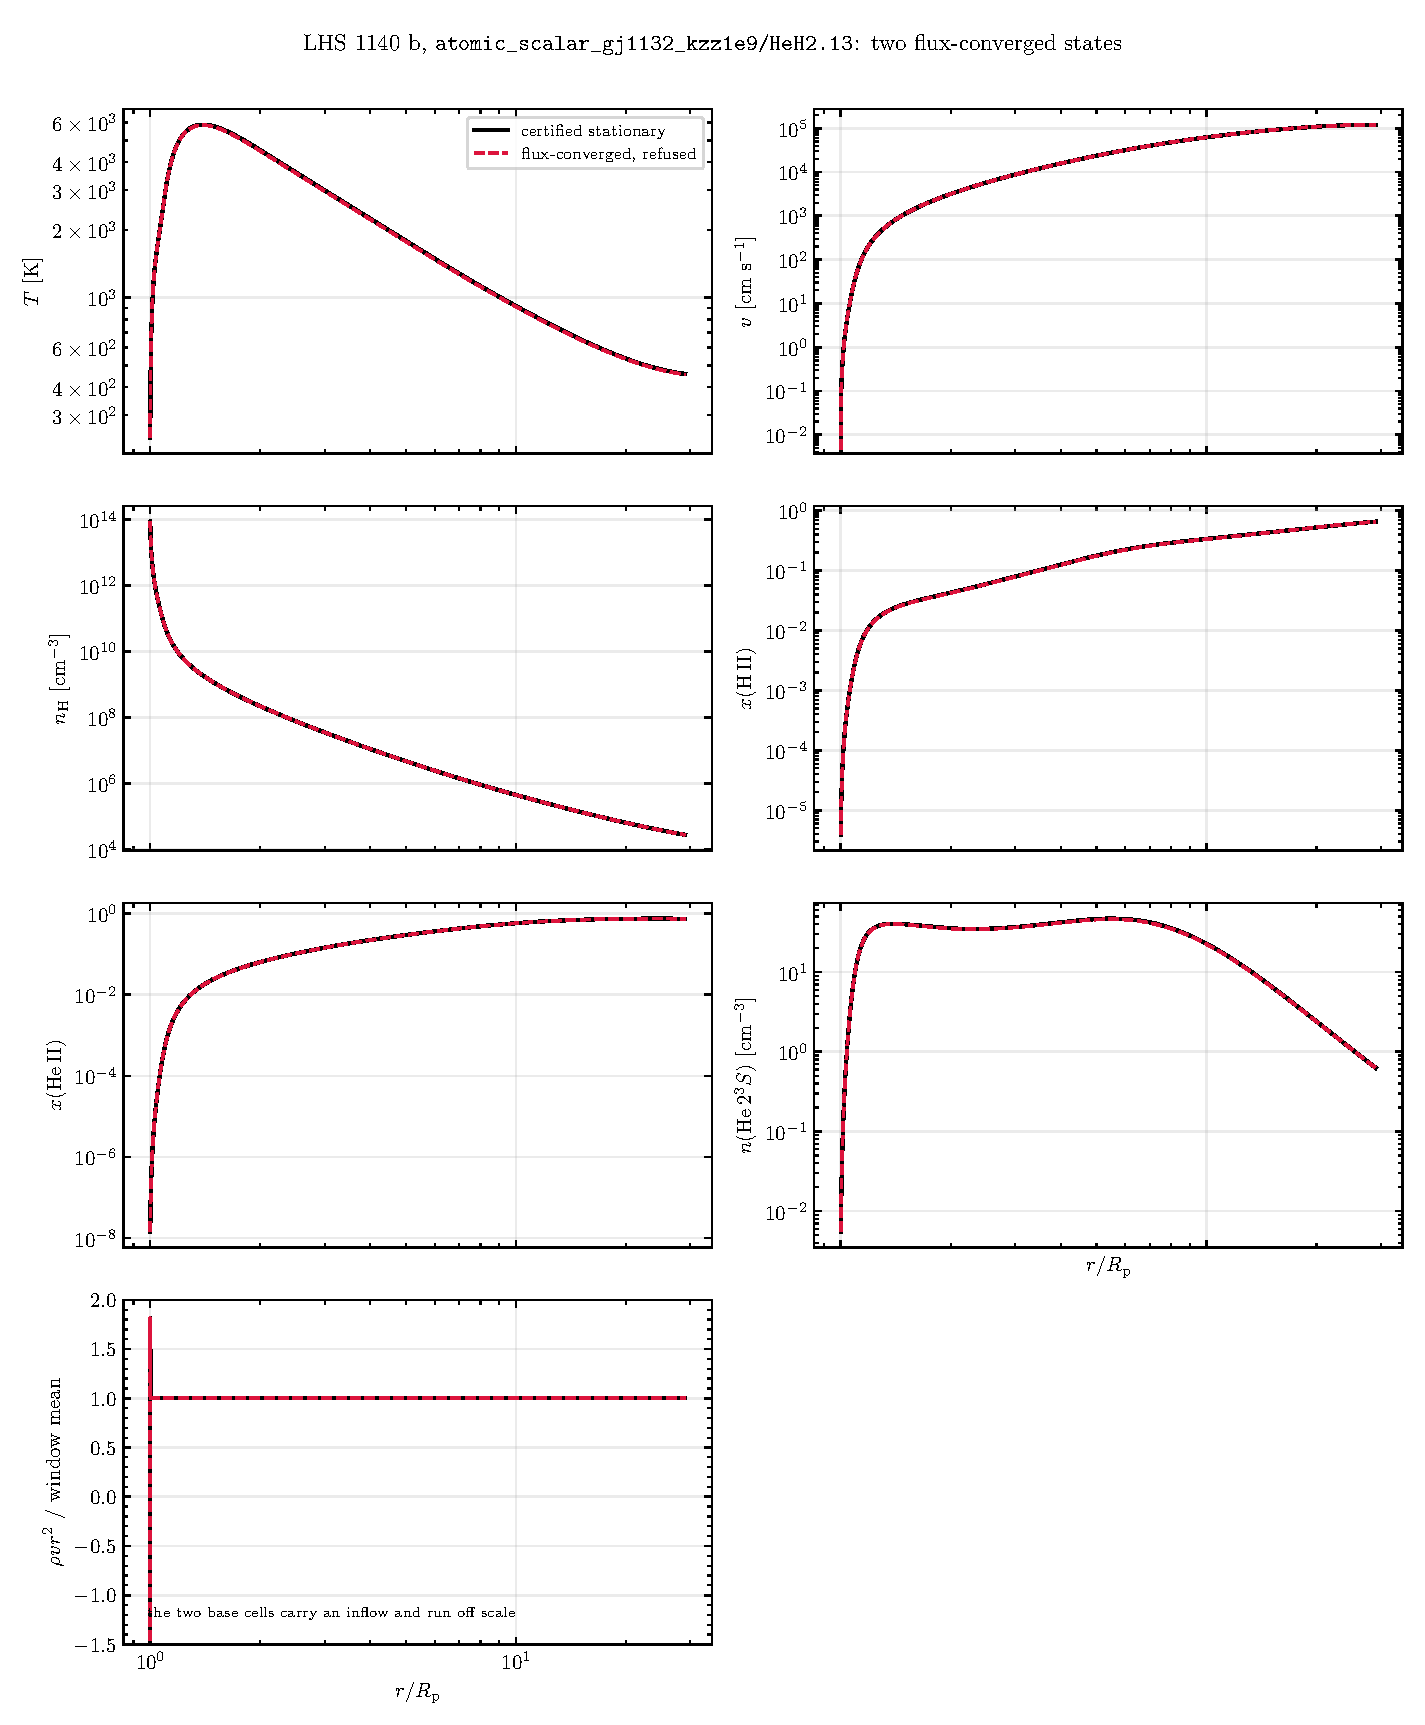
\includegraphics[width=\textwidth]{figures/du_stop_vs_stationary_profiles.pdf}
\caption{The certified stationary solution and the flux-converged refused
state of the atomic \texttt{scalar\_kzz1e9/HeH2.13}, as functions of radius.}
\end{figure}

\begin{figure}[htbp]
\centering
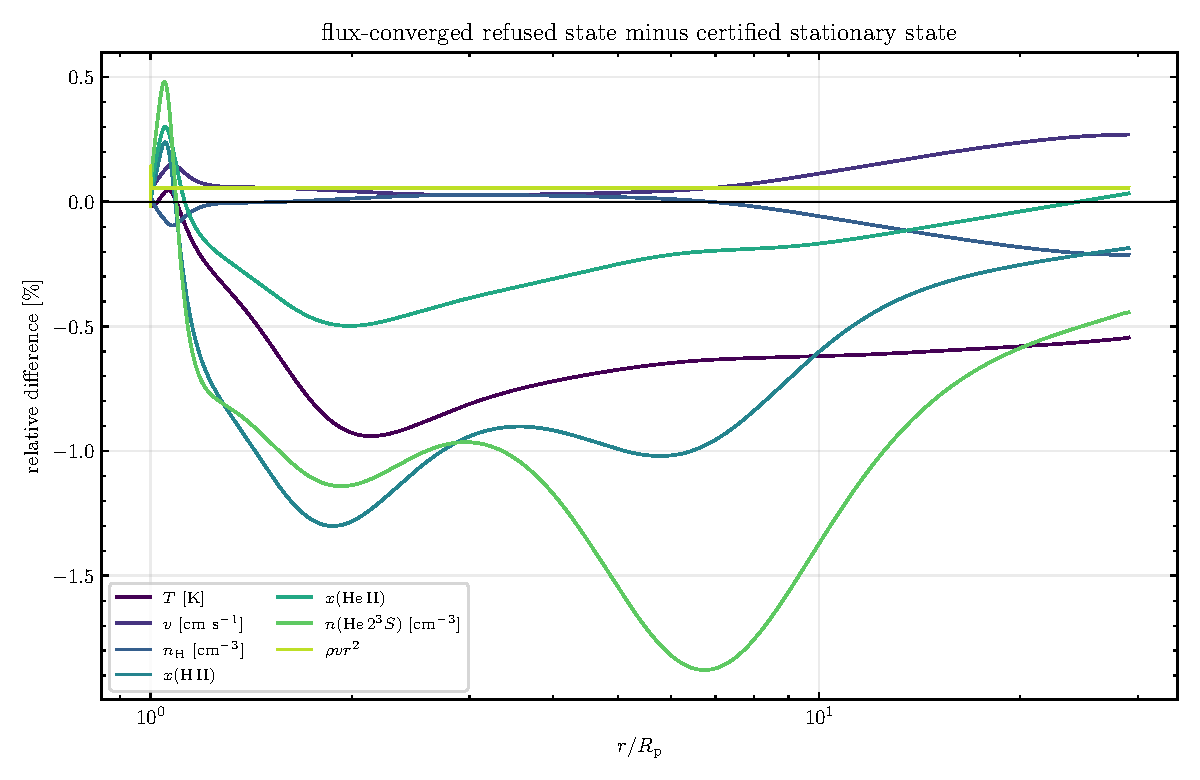
\includegraphics[width=\textwidth]{figures/du_stop_vs_stationary_differences.pdf}
\caption{The same two states, as the relative difference of each quantity.
The largest are the temperature at $r = 2.13\,R_p$ ($-0.94$ per cent),
$x(\mathrm{H\,II})$ at 1.87 ($-1.30$) and $n(\mathrm{He}\,2^3S)$ at 6.74
($-1.88$).}
\end{figure}

\begin{figure}[htbp]
\centering
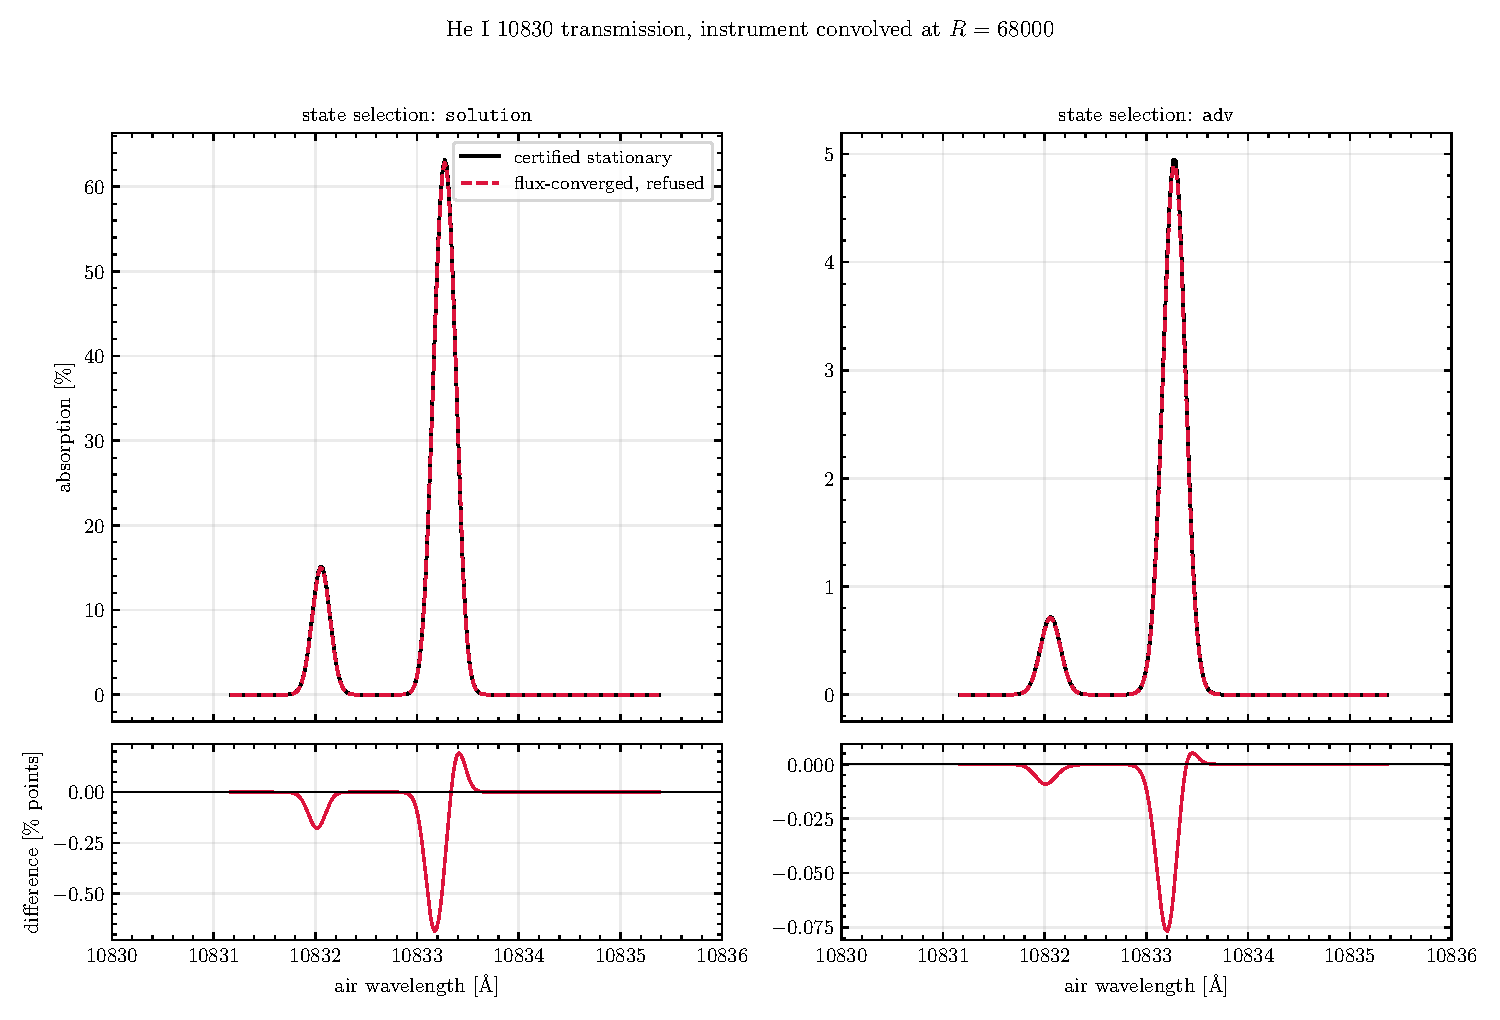
\includegraphics[width=0.85\textwidth]{figures/du_stop_vs_stationary_he10830.pdf}
\caption{The He~I 10830 transmission of the two states.}
\end{figure}

\end{document}
